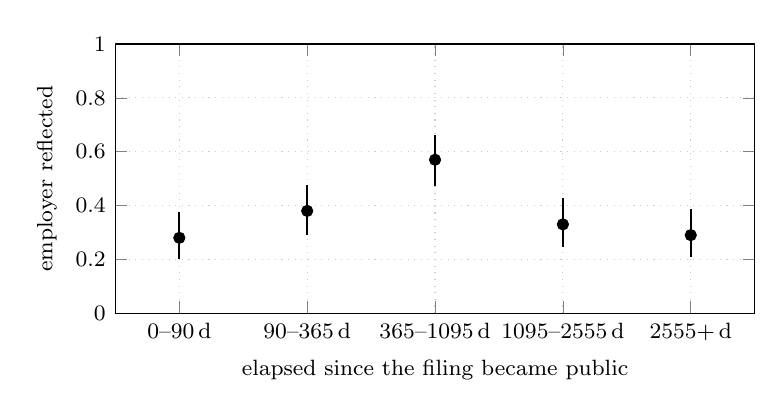
\begin{tikzpicture}
\begin{axis}[width=0.8\linewidth,height=5cm,xlabel={elapsed since the filing became public},ylabel={employer reflected},xtick={1,2,3,4,5},xticklabels={0--90\,d,90--365\,d,365--1095\,d,1095--2555\,d,2555+\,d},ymin=0,ymax=1,xmin=0.5,xmax=5.5,grid=major,major grid style={dotted,gray!40},tick label style={font=\footnotesize},label style={font=\footnotesize}]
\addplot[black,thick] coordinates {(1,0.2014) (1,0.3749)};
\addplot[black,thick] coordinates {(2,0.2910) (2,0.4779)};
\addplot[black,thick] coordinates {(3,0.4722) (3,0.6627)};
\addplot[black,thick] coordinates {(4,0.2456) (4,0.4269)};
\addplot[black,thick] coordinates {(5,0.2101) (5,0.3854)};
\addplot[only marks,mark=*,black] coordinates {(1,0.2800) (2,0.3800) (3,0.5700) (4,0.3300) (5,0.2900)};
\end{axis}
\end{tikzpicture}
